\documentclass{article}

\usepackage[english]{babel}
\usepackage[letterpaper,top=2cm,bottom=2cm,left=3cm,right=3cm,marginparwidth=1.75cm]{geometry}
\usepackage{amsmath}
\usepackage{graphicx}
\usepackage[colorlinks=true, allcolors=blue]{hyperref}

\title{QuickLit: An LLM-Assisted System for Literature Retrieval, Summarization, and Exploration}
\author{Ziyue Gong 1005710740
\and Yuanrong Han 1010787409}

\begin{document}
\maketitle
\section*{Permissions}
\begin{tabular}{|l|c|c|c|}
\hline
\textbf{Group Member} & \textbf{Post Video} & \textbf{Post Final Report} & \textbf{Post Source Code} \\ \hline
Ziyue Gong       & Yes & Yes & Yes \\ \hline
Yuarnrong Han    & Yes & Yes & Yes \\ \hline
\end{tabular}

\section*{Word Count}
1959 words (excluding references, tables, figures, and captions)

\newpage
\section{Introduction}
The motivation for our project is to reduce the manual grind of finding and skimming papers—by automating retrieval and summarization with LLMs—so users can quickly see which papers matter and why.
Thus, our goal is to develop an agentic system that automates the literature retrieval, summarization, and understanding workflow—specifically, the system 
(1) retrieves relevant papers given a research topic; 
(2) summaries extend beyond abstracts and conclusions;
(3) provides an integrated chatbot for users to explore the literature interactively.

Given a research topic such as ``Security Risk and Attacks in AI'' or ``Graph Retrieval--Augmented Generation for Large Language Models, the system automatically constructs structured search queries, retrieves arXiv papers, filters them using semantic similarity, and returns a ranked list with stable \texttt{(paper\_id, title, pdf\_url)} triples.
On demand, QuickLit can then summarize individual papers at the section level and support interactive chat grounded in the retrieved corpus using a retrieval-augmented generation (RAG) pipeline.

\section{Background}
Elicit is a closely related system with similar goals—natural-language querying, ranked retrieval, conversational interaction, and summarization\cite{kung2023elicit}\cite{bernard2025elicit}. However, it offers stronger cross-paper synthesis (e.g., structured matrices, export tools, and auto-generated literature reviews). In comparison, QuickLit currently focuses on retrieval and section-level summarization rather than deeper synthesis.

An external study evaluating Elicit in AI-assisted literature workflows highlights repeatability, human-rated accuracy for one topic, and screening reliability \cite{bernard2025elicit}. QuickLit also measures accuracy, but via cosine similarity across multiple topics. Adding a repeatability check—such as the stability of top-k results—would better align with that framework.

Both systems share limitations: they lack access to paywalled content, and they can query only via Semantic Scholar and QuickLit via arXiv. While effective for rapid scoping, both still require human screening for final relevance, especially since Elicit can occasionally autocorrect queries (e.g., “ontology’’ → “oncology’’). 

A final note that we discovered Elicit only after completing QuickLit. The alignment in objectives and workflow retrospectively validates our system design and highlights the broader demand for AI-supported literature discovery and evaluation tools.


\section{Data and Labels}
\subsection{System I/O Data}
QuickLit ingests and emits the following:
\begin{itemize}
\item \textbf{Input (query):} a research topic.
\item \textbf{Output (retrieval):} up to 30 arXiv papers per topic, each with title, URL, abstract, and an on-demand summary.
\item \textbf{Input (follow-up questions to chatbot):} questions about the retrieved papers.
\item \textbf{Output (chatbot answers):} responses that quote relevant parts of the retrieved papers.
\end{itemize}

\subsection{Evaluation Data and Labels}
See Section Metrics of Success.
\section{Architecture and Software}

\subsection{High-Level System Architecture}
\begin{figure}[h]
    \centering
    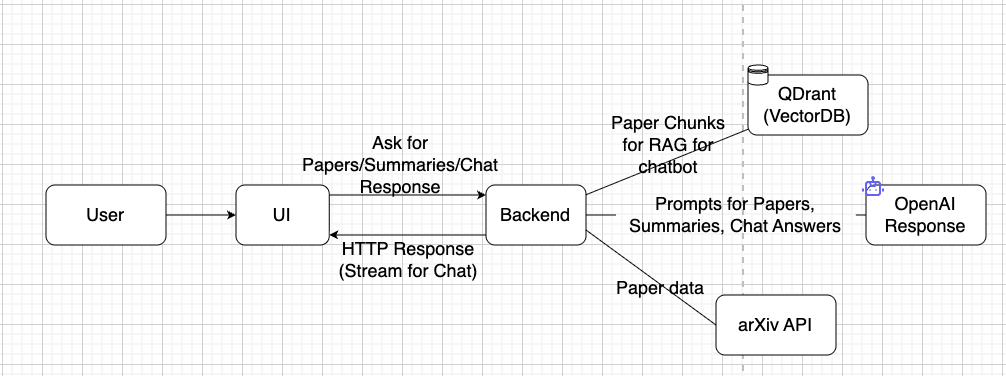
\includegraphics[width=\linewidth]{./image/high level.png}
    \caption{High-Level System Architecture}
    \label{fig:high level}
\end{figure}

QuickLit is deployed as a web application with three main components. Figure~\ref{fig:high level}.
\begin{itemize}
  \item \textbf{Frontend}: a web UI (in \texttt{quicklit-web/}) that allows users to enter topics, browse retrieved papers, request summaries, and chat with an assistant grounded in selected papers.
  \item \textbf{Backend API}: a FastAPI application that exposes endpoints for querying papers, building Qdrant collections, running RAG queries, streaming chat completions, and generating summaries.
  \item \textbf{Vector store}: a Qdrant instance used to store chunked paper text and enable semantic retrieval for the RAG chatbot.
\end{itemize}
The entire system is orchestrated with Docker Compose, with separate containers for the frontend, backend, and Qdrant.
Environment variables configure the OpenAI API key and Qdrant host/port.

\subsection{Retrieval Pipeline}
\begin{figure}[h]
    \centering
    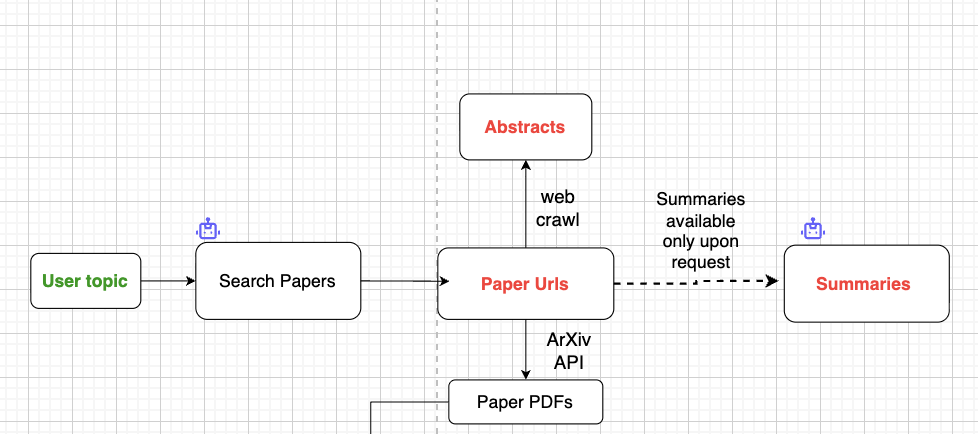
\includegraphics[width=\linewidth]{./image/retrieval.png}
    \caption{Paper Retrieval Pipeline}
    \label{fig:Paper Retrieval Pipeline}
\end{figure}
Given a topic, the retrieval pipeline follows the sequence illustrated in Figure~\ref{fig:Paper Retrieval Pipeline}:

\begin{enumerate}
    \item A search agent (\texttt{gpt-5}) searches for papers by extracting core concepts, forming structured queries, and retrieving arXiv paper triples (\texttt{id, title, url}).
    \item The system crawls abstracts using the URLs.
    \item When requested by the user, the URL is passed to a summary-generation agent (\texttt{gpt-5}) to produce section-level summaries.
    \item Full-text PDFs are fetched using the same URLs and ingested into the vector database for downstream chat.
\end{enumerate}

\subsection{RAG and Chat Pipeline}
\begin{figure}[h]
    \centering
    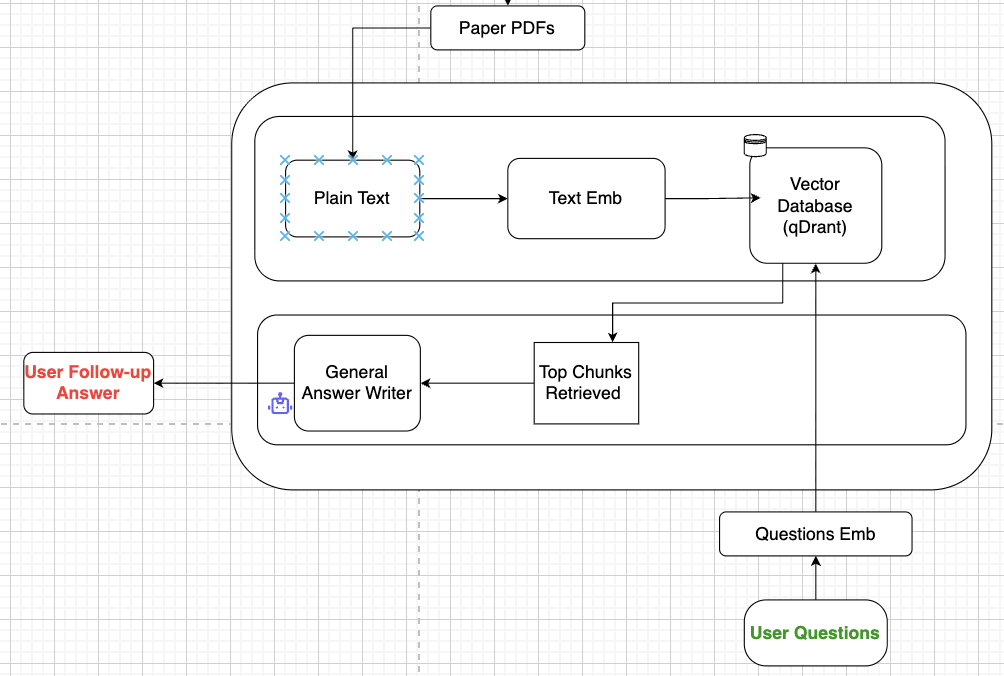
\includegraphics[width=\linewidth]{./image/chat.png}
    \caption{RAG and Chat Pipeline}
    \label{fig:RAG and Chat Pipeline}
\end{figure}
Once papers are retrieved,
\begin{enumerate}
  \item Fetch papers and convert to plain text.
  \item Split and embed text, store in a Qdrant vector database along with chunk metadata.
\end{enumerate}

Once a user inputs a question:
\begin{enumerate}
  \item The question is embedded and used to query Qdrant for the top--$k$ most relevant text chunks.
  \item These retrieved chunks and the user’s question are passed to a general answer-writing LLM (\texttt{gpt-5}).
  \item The LLM synthesizes an answer and returns it to the user.
\end{enumerate}

\section{Metrics of Success}
 We report metrics for retrieval, summarization, RAG-based ranking, and chat quality.

\subsection{Retrieval Metrics}
\textbf{Data.} Gathered papers for 5 versions of prompts, for each of 5 evaluation topics: (1) Deep Reinforcement Learning for Data Processing and Analytics, (2) Security Risk and Attacks in AI, (3) Graph Retrieval--Augmented Generation for Large Language Models, (4) Machine Learning Approaches and Its Techniques, and (5) Edge Computing Systems and Tools.

\textbf{Metrics.}
\begin{itemize}
  \item Mean and median cosine similarity between the topic embedding (using model: all-MiniLM-L6-v2) and each paper's embedding (title and abstract).
  \item Precision of retrieved papers with cosine similarity $\geq 0.4$.
  \item Top-10 precision at threshold $\geq 0.4$.
\end{itemize}

\textbf{Success Criterion.} We refer to an external benchmark for all-MiniLM-L6-v2: In the QT (Question Target) corpus for clinical question answering, cosine similarity among highly relevant abstracts ranges from \textbf{0.59--0.90} (FQ1) and \textbf{0.55--0.99} (FQ2)~\cite{info2023minilm}.

\subsection{Summarization Metrics}

\textbf{Data:} Section-level summaries were generated for three arXiv papers (2504.00761, 2506.09159, 2510.09851). Each paper includes arXiv metadata and a parsed PDF URL.

\textbf{Metrics:} An LLM judge assigns 1--10 scores for:
\begin{itemize}
  \item Section coverage: covers all first-level sections. Captures the core ideas of each section. 
  \item Concision: each section is concise while maintaining clarity and completeness.
  \item Faithfulness: ideas mentioned in the summary have direct references in the original paper.
  \item Writing quality: grammar, clarity, coherence.
  \item Overall quality: weighted holistic score.
\end{itemize}

\textbf{Success Criterion.} Summaries scoring $\geq 8$ in coverage and faithfulness; concision and writing quality are secondary.

\subsection{Mean Reciprocal Rank for RAG Retrieval}
We use Mean Reciprocal Rank (MRR) to quantify how well the RAG retriever surfaces the correct paper near the top of the ranked list. For a given query, let $r$ be the rank (1 for top result, 2 for second, etc.) of the first retrieved chunk whose \texttt{paper\_title} matches the true target paper; the reciprocal rank is then $\mathrm{RR} = 1/r$, and it is $0$ if the target never appears in the top-$k$. Across a set of queries $Q$, the mean reciprocal rank is
\[
\mathrm{MRR@}k = \frac{1}{|Q|} \sum_{q \in Q} \mathrm{RR}(q).
\]

The script \texttt{backend/eval/retrieve\_eval/eval\_mrr.py} evaluates this for three held-out arXiv papers. It downloads each paper, parses the PDF into text, chunks the content, and stores it in a dedicated Qdrant collection, then issues four natural-language queries per paper (asking for its summary, key contributions, methods, and problem statement). For each query, it calls \texttt{query\_qdrant\_openai} with \texttt{top\_k = 10}, computes the reciprocal rank using the helper \texttt{reciprocal\_rank}, and finally reports the overall $\mathrm{MRR@10}$ along with per-query RR values. Running this script end-to-end thus provides an automated regression test of RAG retrieval quality.

\textbf{Data Collected} Three arXiv papers (2511.04213, 2511.01956, 2511.03070) were ingested as parsed chunks (abstract + PDF). For each paper, four query variants were asked: (1) ``summary of \{title\}'', (2) ``key contributions of \{title\}'', (3) ``methods used in \{title\}'', and (4) ``which problem \{title\} addresses''. Evaluation is under \texttt{backend/app/eval\_mrr.py}.

\subsection{Chat Metrics}

\textbf{Data} User follow-up questions paired with grounded chatbot answers, scored by model-based evaluators.

\textbf{Rubric (agentic judge).} Weighted scoring over five dimensions:
\begin{itemize}
  \item Grounding accuracy (0.35),
  \item Responsiveness (0.20),
  \item Evidence and citation quality (0.15),
  \item Reasoning quality (0.15),
  \item Communication and safety (0.15).
\end{itemize}

\textbf{Metric.} The final chat score is a weighted sum on a scale of 0-5.



\section{Quantitative Results}
\subsection{Retrieval Results}

We evaluate retrieval performance across five query pipelines—two semantic baselines and three arXiv-only variants—using mean cosine similarity as the primary metric. Table~\ref{tab:retrieval} reports the mean similarity scores for the most recent arXiv-only pipeline (v5 in \texttt{compare\_scores.csv}) across the five evaluation topics.

\begin{table}[h]
\centering
\begin{tabular}{l|c}
\textbf{Topic} & \textbf{Mean similarity (v5)} \\\hline
Deep RL for Data Processing and Analytics & 0.45 \\
Security Risk and Attacks in AI           & 0.40 \\
Graph Retrieval--Augmented Generation     & 0.60 \\
Machine Learning Approaches               & 0.25 \\
Edge Computing Systems and Tools          & 0.52 \\
\end{tabular}
\caption{\label{tab:retrieval}Mean topic--paper similarity for the latest arXiv-only pipeline (v5) across evaluation topics.}
\end{table}

\subsection{Summary Scores}

For a subset of edge--computing papers, we evaluated section--level summaries using the LLM judge rubric.
Table~\ref{tab:summary} shows the resulting scores aggregated in \texttt{combined\_summary\_scores.csv}.

\begin{table}[h]
\centering
\begin{tabular}{l|c|c|c|c|c}
\textbf{Paper (arXiv ID)} & \textbf{Cov.} & \textbf{Conc.} & \textbf{Faith.} & \textbf{Write.} & \textbf{Overall} \\\hline
2504.00761 & 9  & 8 & 9  & 8 & 8.0  \\
2506.09159 & 10 & 8 & 10 & 9 & 9.0  \\
2510.09851 & 10 & 9 & 10 & 9 & 9.5  \\
\end{tabular}
\caption{\label{tab:summary}LLM--judged summary scores (1--10) for three edge--computing papers.}
\end{table}

These scores indicate that the system can produce summaries with near-perfect faithfulness and coverage, and overall scores between 8 and 9.5 without any task-specific supervision.

\subsection{MRR for RAG Retrieval}
For this small RAG sanity check, we ingested three papers on LLM feedback for statistics exams, AI-supported education, and observational benchmarks for LLMs, and issued four natural-language queries per paper (summarizing, listing key contributions, describing the methods, and identifying the problem addressed). For all 12 queries, the correct paper was retrieved at rank~1, yielding a reciprocal rank of $1.0$ for every query and an overall $\mathrm{MRR@10} = 1.000$. This confirms that, once the relevant papers are in the Qdrant collection and the query explicitly references the target title, the RAG retriever reliably surfaces the correct document at the top of the ranked list; more challenging paraphrased queries and larger candidate sets are left for future evaluation.

\subsection{Chat Scores}
We ran the agentic chat evaluator on seven saved conversations in \texttt{backend/eval/chat\_eval/}, spanning single-paper question answering (e.g., SimClass; advantages and disadvantages of ChatGPT in education) and multi-paper synthesis of scoping reviews and policy analyses. Each conversation was scored on a 0--5 scale using the weighted rubric from Section~\textit{Metrics of Success}. Across runs, weighted scores ranged from \textbf{3.0} for early multi-paper summaries using smaller context chunks (with some hallucinated counts and missing citations) up to \textbf{5.0} for runs that reused the same prompts but evaluated chats built from larger chunk sizes. Typical strong conversations achieved weighted scores between \textbf{4.15} and \textbf{4.85}. The judge consistently flagged two main failure modes: incomplete coverage of all included papers and insufficient explicit evidence. Notably, when we switched to larger chunk sizes for the same tasks, hallucination flags disappeared, and weighted scores improved.

\begin{table}[h]
\centering
\small
\begin{tabular}{p{0.4\linewidth} c p{0.28\linewidth}}
\textbf{Scenario} & \textbf{Score} & \textbf{Main issues} \\\hline
Single-paper QA                    & 4.70 & evidence \\
Multi-paper overview  & 3.00 & hallucination, coverage, other \\
Single-paper pros/cons             & 4.15 & coverage \\
Multi-paper focus      & 4.85 & coverage \\
Multi-paper focus (large chunk)      & 5.00 & none \\
Single-paper adv./disadv. & 4.65 & coverage \\
Single-paper adv./disadv. (large chunk)  & 4.85 & none \\
\end{tabular}
\caption{\label{tab:chat-scores}Agentic judge chat scores across saved conversations.}
\end{table}

\section{Qualitative Results}
For paper retrieval, as shown in Table~\ref{tab:retrieval}, two topics: "Graph Retrieval--Augmented Generation" and "Edge Computing Systems and Tools" achieve mean similarities near or above \textbf{0.50} and also exhibit \textbf{top-10 precision of 1.0}. These scores fall within the QT reference range, indicating good retrieval. In contrast, broad or underspecified queries such as ``Machine Learning Approaches’’ produce substantially lower similarity \textbf{0.25}. This mirrors the behavior observed in the QT corpus, where similarity decreases when queries become less specific or more heterogeneous. 


On the summarization side, manual inspection of the MOSE paper shows that the generated section-by-section summaries correctly identify system components, experimental setups, and key results, such as improvements in migration latency and service availability, without inventing non-existent baselines or metrics.
The LLM judge's explanations corroborate this, highlighting that the summaries ``cover all primary sections'' and ``preserve nuance'' from both benefits and limitations sections.

For chat, example traces show that the agentic judge rewards answers that enumerate both advantages and disadvantages of LLMs in education, grounding each point in specific cited works (e.g., surveys on LLM usage in postgraduate education), and penalizes responses that omit key trade-offs or fail to reference the underlying literature.

\section{Discussion and Learning}

A key lesson learned was the importance of selecting evaluation metrics. Our initial paper retrieval metric—title matching against survey-derived citation lists—proved ineffective, not because the system retrieved poor papers, but because the gold lists did not comprehensively cover each topic. Later, we switched to metrics grounded in prior literature: embedding-based cosine similarity, which offered clearer interpretability and more stable signals.

We also observed practical limitations of the agentic system: it can be slow and non-deterministic, producing minor variations across runs. Browser-level caching helped mitigate this, and future work will explore lighter or more deterministic models to support reproducible evaluation.

Also, adding a small set of human-labeled summaries and chat ratings could help calibrate our metrics. We also aim to explore diversification objectives in retrieval, ensuring coverage across subtopics rather than ranking solely by text similarity. 


\section{Individual Contribution}
\textbf{Ziyue Gong}
\begin{itemize}
    \item \textbf{Paper Retrieval}: Designed and iterated the retrieval endpoint across five prompt versions (Scholar Semantic API → arXiv v3–v5); implemented evaluation for five topics across all versions and aggregated results into comparison tables.

    \item \textbf{Summarization}: Implemented the summary-generation endpoint; designed and ran an LLM-judge–based evaluation for three summaries.
\end{itemize}

\noindent\textbf{Yuanrong Han}

\begin{itemize}
    \item \textbf{System Deployment}: Set up Docker-based containerization for the Qdrant vector store, backend API, and React frontend, and maintained the Compose configuration for local development.
    \item \textbf{Frontend Implementation}: Initialized the QuickLit web frontend and refactored the React components and layout to support topic search, paper browsing, and summary display.
    \item \textbf{RAG and Chat Pipeline}: Built the retrieval-augmented generation pipeline connecting retrieval, Qdrant, and the LLM, and implemented the chatbot backend and UI flow for grounded question answering over selected papers.
\end{itemize}

\bibliographystyle{IEEEtran}
\bibliography{sample}

\end{document}
